
\chapter{Smoluchowski}

{
\color{red}
\begin{itemize}
\item Fokker Planck, SDE
\item on whole $\mathbb R$, do box $[-L,L]^d$, Neuman / Dirichlet BC?
\item instead solve for $q=\ln(p)$ ?
\item benchmark for:
\item - $\int p = 1$
\item - convergence to equilibrium $e^{-V(x)}$
\item - capture relatively sharp features
\item - probabilities become 0 very quickly in high dim space

\item sampling - importance sampling from distribution / sde
\item add prob = 1 loss?
\item sampling via sde + lhs

\end{itemize}

}


\section{Formulation}

Diffusion in the present of forces.
If force given by some potential V -> smoluchowksi.\cite{kneller}
Many particle system - more particles.
Here, non interacting case as interactions hard for SG to implement - no comparison.

confining potential, particle bound and not escape to infinity

analytic not known but equlibrium yes

super fast conv to equilibrium - if V satisfied in L and V to inf when x to inf 
\cite{pavliotis}


Consider the motion of an overdamped Brownian particle in an external potential $V(x)$ on $\mathbb{R}^d$, whose stochastic differential equation has the form

$$
dX_t = -\nabla V(X_t)\,dt + \sqrt{2\beta^{-1}}\,dW_t
$$ 
where $\beta = 1/k_b T$, and $k_B$ is the Bolztman constant.

The corresponding probability density $\rho(x,t)$ then satisfies the so-called Smoluchowski equation.
$$
\partial_t \rho = \beta^{-1}\Delta\rho + \nabla\cdot\bigl(\rho\nabla V\bigr)
$$
%linear drift-diffusion eq, 
%mass-conserving convection-diffusion equation
$$
\partial_t\rho = -\nabla\cdot J,\qquad J(\rho) = -(\beta^{-1}\nabla\rho + \rho\nabla V)
$$ 
PDE lives on $\mathbb R^d$.


If $V$ is confining, that is:
$$
\lim_{|x|\to\infty}V(x)=+\infty\quad \text{and} \quad e^{-\beta V}\in L^1
$$

then there exists a unique stationary solution in the form of a Boltzman density
$$
\rho_\infty(x) = \frac{1}{Z} e^{-\beta V(x)} \qquad Z=\int_{\mathbb R^d}e^{-\beta V(x)}dx
$$ 

%\subsection{Properties to exploit / address}
%- linear
%- positivity (max-principle)
%- self-adjoint (reversible)
%- known equilibrium distrib
%- mass conversion
%- energy based approaches?
%- schoedinger type operator?


\subsection{Boundary conditions}
truncate $\mathbb{R}^d$ to a hypercube $[-L,L]^d$.

\textbf{Dirichlet (reactive / absorbing)}

$$
\rho(x,t)=0\quad\text{on}\:\:\partial\Omega
$$
The boundary acts as a perfect sink 
prop decays with time to 0 in the entire Rd\cite{pavliotis}

\textbf{Neumann (no-flux / reflecting)}

$$
(\beta^{-1}\nabla\rho+\rho\nabla V)\cdot n = -J(\rho)\cdot n = 0
\quad\text{on}\:\:\partial\Omega
$$
Particles are reflected, strictly conserving total mass. 
prop stays 1 in entire Rd\cite{pavliotis}

\subsection{Initial conditions}

localized non-equilibrium Gaussian distribution localized at $x_0$:
$$\rho(x, 0) = \left( \frac{1}{2\pi \sigma^2} \right)^{d/2} \exp\left( -\frac{\|x - x_0\|^2}{2\sigma^2} \right)$$


\section{Variants of $V(x)$}


\subsection{Double well}

$$
V(x) = \frac{1}{4}\sum_{i=1}^d (x_i^2-a_i^2)^2
$$
The resulting equilibrium $\rho_\infty\propto e^{-V}$ has $2^d$ well.

%BTW: computing the partition function
%
%$$
%z = \int_{(-\infty,\infty)^d} e^{-\beta V(x_1,...,x_d)} dx_1...dx_d \\
%= \prod_{i=1}^d \left( \int_{-\infty}^\infty e^{-\frac{\beta}{4} (x_i^2-a_i^2)^2} dx_i \right)
%$$
%
%we uniformly sample $a_i$ from the interval $(0.85,1.15)$
%
%choosing L = 3.5 is enough
%
%using numpy's polyfit, we get
%$$
%\int_{-\infty}^\infty e^{-\beta (x^2-a^2)^2} dx \approx -1.048 a^3 + 1.618 a^2 + 0.03337 a + 2.438 =: z_{fit}(a)
%$$



\subsection{Coupled double well}

\begin{equation}
V_{\text{DW-cpl}}(x)=\sum_{i=1}^d \frac{1}{4}(x_i^2-a^2)^2+\frac{\gamma}{2}\sum_{i=1}^{d-1}(x_{i+1}-x_i)^2,\qquad \gamma\ge 0.
\tag{V-DWC}
\end{equation}

The coupling parameter $\gamma$ -> no separability.

\subsection{xAx}
$$
V(x)=\tfrac12 x^T A x
$$
with a positive-definite matrix $A$.
In coordinates smthg like
$V(x)=\sum_i \alpha_i x_i^2 + \sum_{i\ne j} \gamma_{ij}x_ix_j$.


\subsection{Rastrigin}

classic “many-minima” test function adapted as a potential.

\begin{equation}
V_{\text{Rast}}(x)=A d+\sum_{i=1}^d\left(x_i^2-A\cos(2\pi x_i)\right),\qquad A>0.
\tag{V-R}
\end{equation}



\textbf{See next page for a visualizations}


\begin{figure}
    \centering
    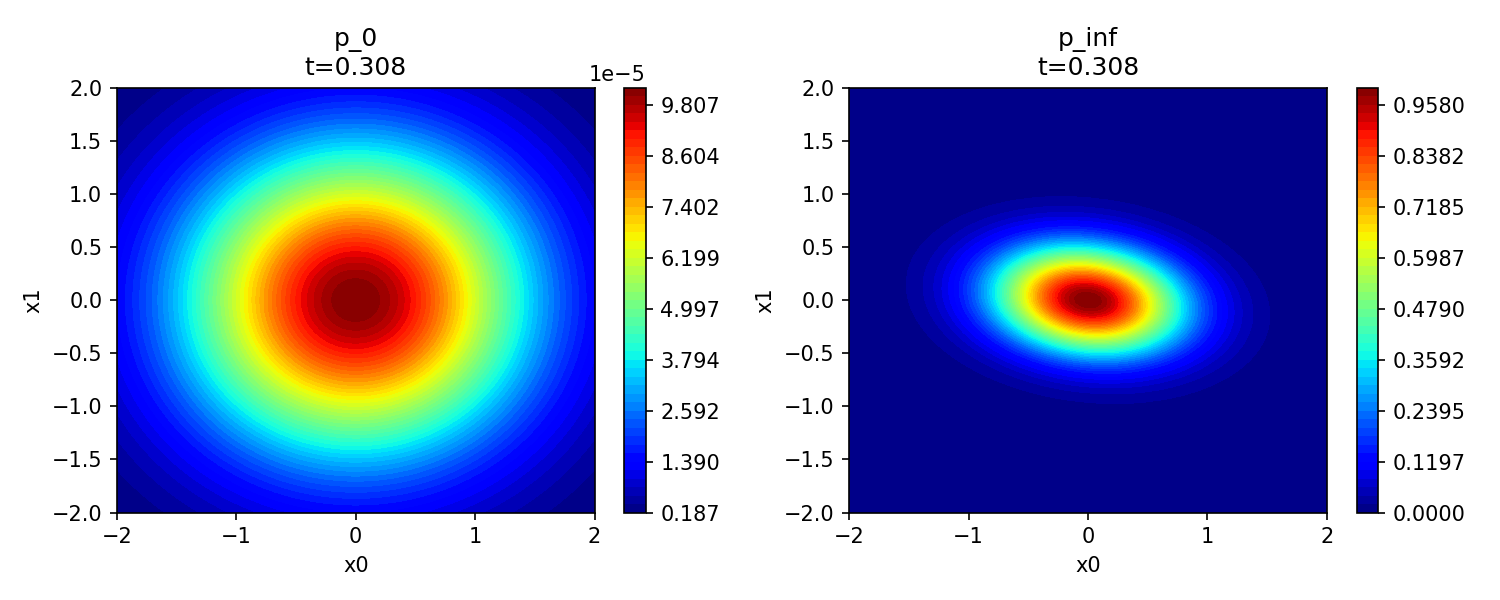
\includegraphics[width=\linewidth]{figures/V=QP.png}

    \medskip
    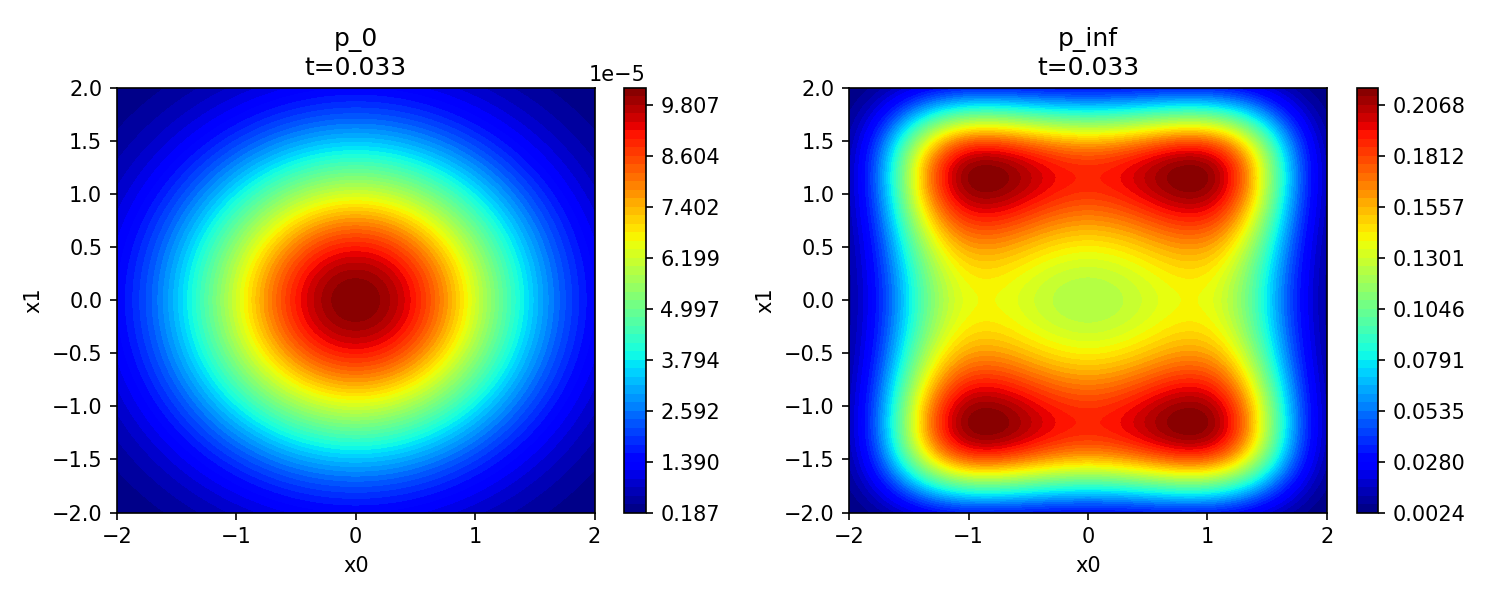
\includegraphics[width=\linewidth]{figures/V=DW.png}

    \medskip
    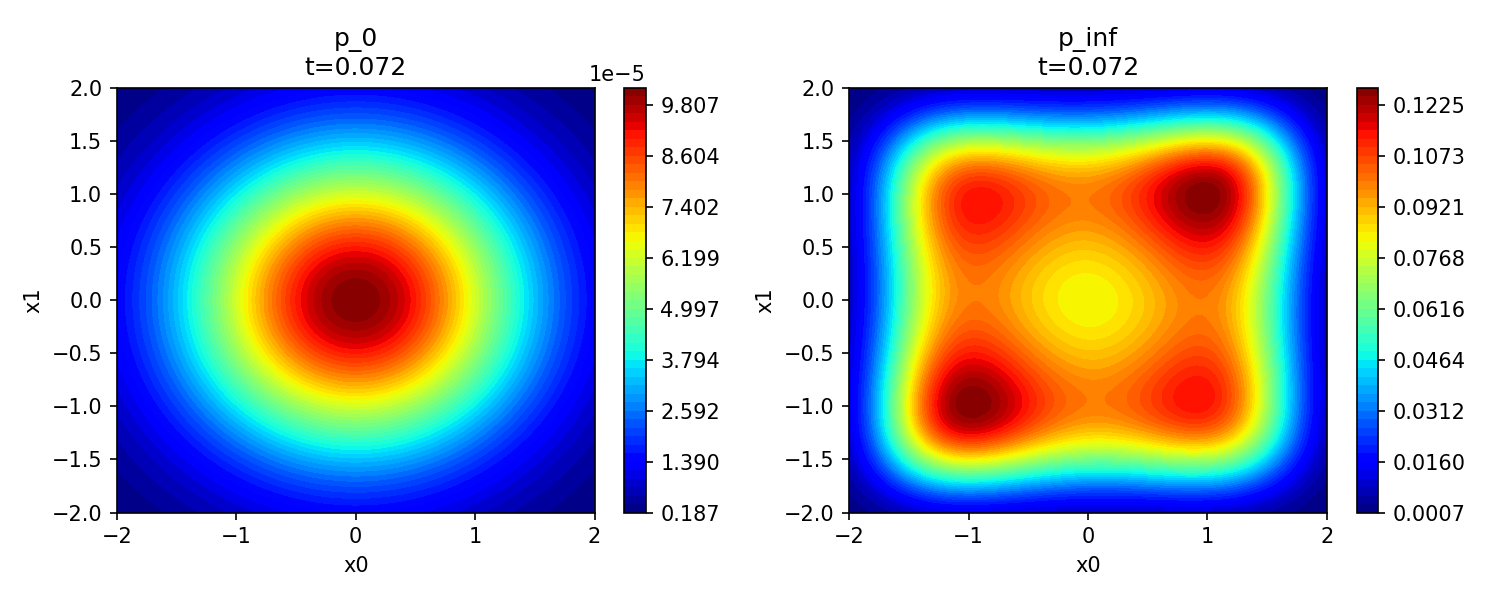
\includegraphics[width=\linewidth]{figures/V=CDW.png}

    \medskip
    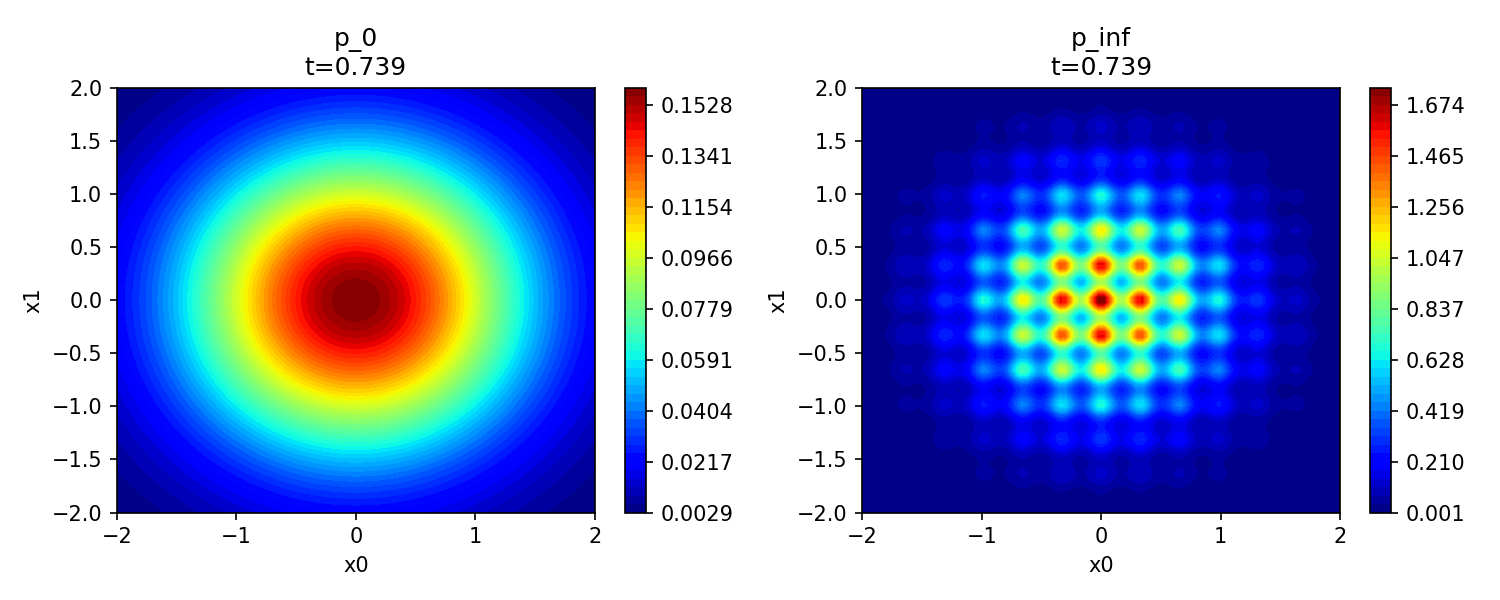
\includegraphics[width=\linewidth]{figures/V=Rastigin.png}
    \caption{(left): initial condition - unit gaussina, (right): $e^{-\beta V(x)}\,,\: V(x)=$ Quadratic pot, Double Well, Coupled Double well, Rastrigin}
\end{figure}



\section{Sparse grid combination technique}

neumann?


\subsection{2-dimensional calibration case}


\section{PINNS}

In all the experiments below, we consider:

\begin{itemize}
\item learning rate (lr) of 1e-3
\end{itemize}

Due to the stochastic nature of the equaiton,
- lhs 1/2 points
- sde 1/2 points - random in domain from 100 trajectories, for 1000 steps, pick random

More localized features - silu activation funciton.

The reported $L^\infty$ and relative $L^2$ erros are both computed form a collection of
100,000 points sampled using the LHS throughout the entire spatial-temporal domain.
again, the $L^\infty$ is given as $\max(L^\infty_{pde}, L^\infty_{ic})$, and
the relative $L^2$ error as the average of the corresponding PDE and IC relative $L^2$ errors.


sample 10k,100k etc. the IC based on ic gaussian - importance sampling to cover high imporance regions
sample 10k,100k etc. the TS based on tc e-V - importance sampling to cover high imporance regions
sample 10k, 100k, distributed at the 4 additioanl time slices
- prepare samples using SDE
save all sets, reuse in SG

testing performed at high magnitude points
- time windows

\subsection{2-dimensional calibration case}

Same model as in heat eq:
\begin{center}
\begin{tabular}{ |c|c|c|c } 
\hline
NN size & steps & number of collation points, or batch size (bs)\\
\hline
4x64  & 10,000 & 1024 \\
\hline
\end{tabular}
\end{center}
where by '4x64' we again, mean a neutral network with 4 hidden layers,
each consisting of 64 neurons.

Based on results from prev chapter on heat eq:
- Expomential lr decay, with a frequncy of 25 times during the training.
- bs = 1024
- more lambdas? use gradadapt

Also, the collations points for the initial and bc conditon is 8 times less than that for pde.

%%%%%%%%%%%%%%%%%%%%%%%%%%%%%%%%%%%%%%%%%%%%%%%%%%%%%%%%%%%%%%
% TRY 2D:
- class PDE and \texttt{q\_pde}
- 3,4 layers
causal struct more pronounced - quite diff struct in time
- causal sampl
- time loss weight
- neuma dirichlet

%%%%%%%%%%%%%%%%%%%%%%%%%%%%%%%%%%%%%%%%%%%%%%%%%%%%%%%%%%%%%%
% Expectations d=2

1e-3 IC / BC err at 10k 20k epochs
not bad
relatively good results
small network

not trained well?

A) prob the issue?
- add to loss?
- loss diff scales?

B) underflow the issue?

C) BC the issue?
- dropping the bc leads to better results?
- sort of hard constrians by mult by gaussian / add log for q pde setup?

%%%%%%%%%%%%%%%%%%%%%%%%%%%%%%%%%%%%%%%%%%%%%%%%%%%%%%%%%%%%%%
% Expectations d larger

depth / width scale in nn params

diff bs


%%%%%%%%%%%%%%%%%%%%%%%%%%%%%%%%%%%%%%%%%%%%%%%%%%%%%%%%%%%%%%
% Results d=2

\subsection{Decay towards 0}

for lambda same and dirichlet condition

result:
solution goes to 0
even the ic is very small - peak of 0.01 compared to 0.15

hypothesis:
- this satisfies both the dirichlet bc and the pde
- so: boundary leaking mass.... ?

solution:
enforce no flux neuman bc??
- but it still goes to zero, since p=0 also satisfies the neuman bc

solution:
use gradnomr to figure it out
- just rises lambda bc super more and thus enforeces bc more since then sol 0.0 can be global not just ic and decay

if we want nonzero sol, need to more stronly enforce the ic
-> raise ic to 100

The model is going to zero, the missing constraint is not terminal information. It is mass conservation.
Increasing $\lambda_{ic}$ cannot fix that, because IC only anchors one time slice. It does not constrain the total mass for $t>0$.

The network is satisfying the objective
- it minimizing the ic loss by fitting the initial condition,
and minimizing the pde and bc by very quickly relaxing the zero.
, hence the the objective has to be changed.

thus we have to incorporate mass conservation into the loss.
normalization loss
$$
\ell_{total} = \lambda_{pde}\ell_{pde}
+ \lambda_{bc}\ell_{bc}
+ \lambda_{ic}\ell_{ic}
+ \lambda_{norm}\ell_{norm}
$$


Every step, we randomly select k time slices, and
calculate the nomr using 2024 points for each slices.

This has a huge effect on the mass conversion, but introduces another
parameter to be tuned.

To resolve the relative magnitude of each lambda, we
monitor the losses during the training and set
such lambdas so that the all $\lambda_r \ell_r$
are all on a similar level.
We also adapt gradadapt norm into this process, to check whethet the 
weights do not drift to far from teh initial values,
which would signifu that the weights should changed.

After extensive tuning, from which we will spare the reader,
we arrive at the following optimal values:

\begin{center}
$\lambda_{pde} = 10.0$, $\lambda_{bc} = 100.0$, $\lambda_{ic} = 100.0$, $\lambda_{norm} = 1.0$

\medskip
\begin{tabular}{ |c|c|c| }
\hline
model & steps & number of collocation points, or batch size (bs) \\
\hline
4x64 & 10,000 & 1024 \\
\hline
\end{tabular}
\end{center}

At this points, running the network for 10k steps, finally 
produces a reasonable result.

L inf is not that bad, but rel L2 still too high.
However, the error is still to high,

Even at the more complex regime where the individual batches might be too noisy,
larges batch size does not offer any imporovement.


Expensive - need to sample a large pool of points to estimate the integral over the domain well.
use SDE trajectories and euler majaruma?


importance sampling from initial and final distrib
- for domain

4x64 too small?

rbas only munumizes l inf err - 



moving to log p -> the pde does depend only on laplace and grad q, not on q itself,
thus q+c is also a solution
